\section{Introduction}
\label{sec:introduction}

A probe can name a clinical signal in a representation. The consequential question is whether changing that named direction selectively changes the model's answer. Linear probes are useful because they expose information available to a restricted readout family \citep{alain2017understanding,hewitt2019designing}. Their accuracy alone, however, does not establish that the underlying model uses the decoded property for its task \citep{ravichander2021probing}.

This distinction matters acutely in medical vision-language models (VLMs). A high clinical probe score is easy to read as evidence that a finding is operational inside the model, even though the score may reflect probe capacity, acquisition structure, or information that the downstream computation ignores. Recent medical VLM work traces classification signals across depth \citep{zhu2026lost}, while VLM steering work uses probe vectors to edit visual concepts \citep{theodoridis2026probing}. These lines establish that clinical or visual properties can be read and that internal edits can move outputs. They leave open whether a target probe normal has a \emph{direction-specific} effect when compared with equally strong, clinically meaningful alternatives at the same consumed locus.

We ask a narrow causal question: when a clinical concept is robustly linearly decodable at the final visual block, does its probe normal exert direction-specific influence on the answer? Figure~\ref{fig:evidence-ladder} summarizes the protocol. We first verify the exact final visual block on the model's forward path. At that locus, we fit one capacity-matched probe under a patient split and compare its AUROC with 20 type-to-random-label controls. We then add the unit probe normal to each visual token at a dose proportional to that token's activation norm. Random directions, a coordinate-permutation sham, and fixed unrelated clinical probe normals receive the same dose. The design treats availability, generic perturbation selectivity, and clinical direction specificity as successive evidentiary rungs.

\begin{figure*}[t]
    \centering
    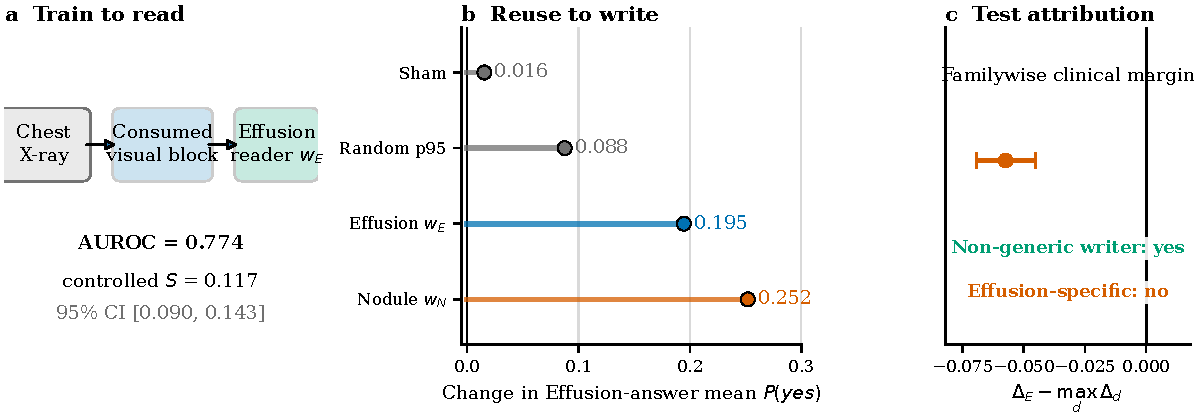
\includegraphics[width=\textwidth]{figures/fig1_evidence_ladder.pdf}
    \caption{\textbf{Decodability, generic perturbation selectivity, and clinical direction specificity are distinct tests.} \textbf{(a)} A fixed-capacity probe reads a clinical label from the exact final visual block consumed downstream; equal-norm interventions edit that same representation. \textbf{(b)} All three registered cells have positive controlled-decoding intervals under patient bootstrap. \textbf{(c)} Filled circles mark passed rungs; crosses mark where a cell stops. LLaVA Effusion and Edema stop at random/sham. Qwen Effusion clears that rung, then stops at fixed clinical directions on an independent 400-patient cohort. Open circles mark rungs not reached by the prospective sequence.}
    \label{fig:evidence-ladder}
\end{figure*}

Our evidence consists of three registered model--concept cells on NIH ChestX-ray14. All three target labels are linearly available, with AUROC between 0.7742 and 0.8009 and positive controlled selectivity. The two LLaVA cells do not clear random/sham controls. Qwen Effusion does clear those controls, including on a prospectively selected cohort of 400 new patients, but the fixed Nodule direction produces a larger response. Its familywise Effusion-minus-maximum-unrelated interval lies entirely below zero.

The paper makes three contributions:
\begin{itemize}
    \item We introduce a forward-path, capacity-controlled protocol that separates controlled decodability, random/sham intervention selectivity, and clinical direction specificity at one consumed representation.
    \item We report three final-block cells in which controlled decodability is positive while the registered direction-specific endpoint is not reached.
    \item We replicate the Qwen behavioural response on independent patients and show that passing random/sham controls is insufficient when a fixed unrelated clinical direction is reliably stronger.
\end{itemize}

The resulting principle is practical: a decoded clinical direction warrants a causal interpretation only after controls test clinical direction specificity at the same locus and dose. Sections~\ref{sec:related}--\ref{sec:protocol} place and define this test, Section~\ref{sec:results} reports the evidence ladder, and Sections~\ref{sec:discussion}--\ref{sec:conclusion} give its interpretation and scope.
